\begin{figure}[htb]
  \centering
  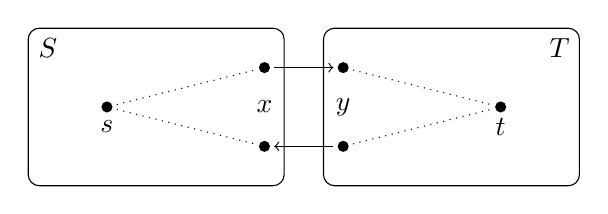
\begin{tikzpicture}
    \node (s) at (2,2) {};
    \node (x1) at (4,2.5) {};
    \node (x2) at (4,1.5) {};
    \node (y1) at (5,2.5) {};
    \node (y2) at (5,1.5) {};
    \node (t) at (7,2) {};
  
    \node at (2,1.75) {$s$};
    \node at (7,1.75) {$t$};
    \node at (4,2) {$x$};
    \node at (5,2) {$y$};
  
    \foreach \node in {s,x1,x2,y1,y2,t}
    {
      \fill (\node) circle(2pt);
    };
    \path (x1) edge[->] (y1);
    \path (y2) edge[->] (x2);

    \path[dotted] (s) edge (x1);
    \path[dotted] (s) edge (x2);
    \path[dotted] (y1) edge (t);
    \path[dotted] (y2) edge (t);

    \node (S) at (1.25,2.75) {$S$};
    \node (T) at (7.75,2.75) {$T$};
    \draw[rounded corners] (1,1) rectangle (4.25,3);
    \draw[rounded corners] (4.75,1) rectangle (8,3);
  \end{tikzpicture}
  \caption{Proof augmented path}
\end{figure}

